\documentclass[border=10pt]{standalone}

\usepackage{tikz}
\usepackage{tikzsymbols}
\usetikzlibrary{calc,patterns,shapes.geometric}

\def\centerarc[#1](#2)(#3:#4:#5){\draw[#1] ($(#2)+({#5*cos(#3)},{#5*sin(#3)})$) arc (#3:#4:#5);}

\begin{document}
	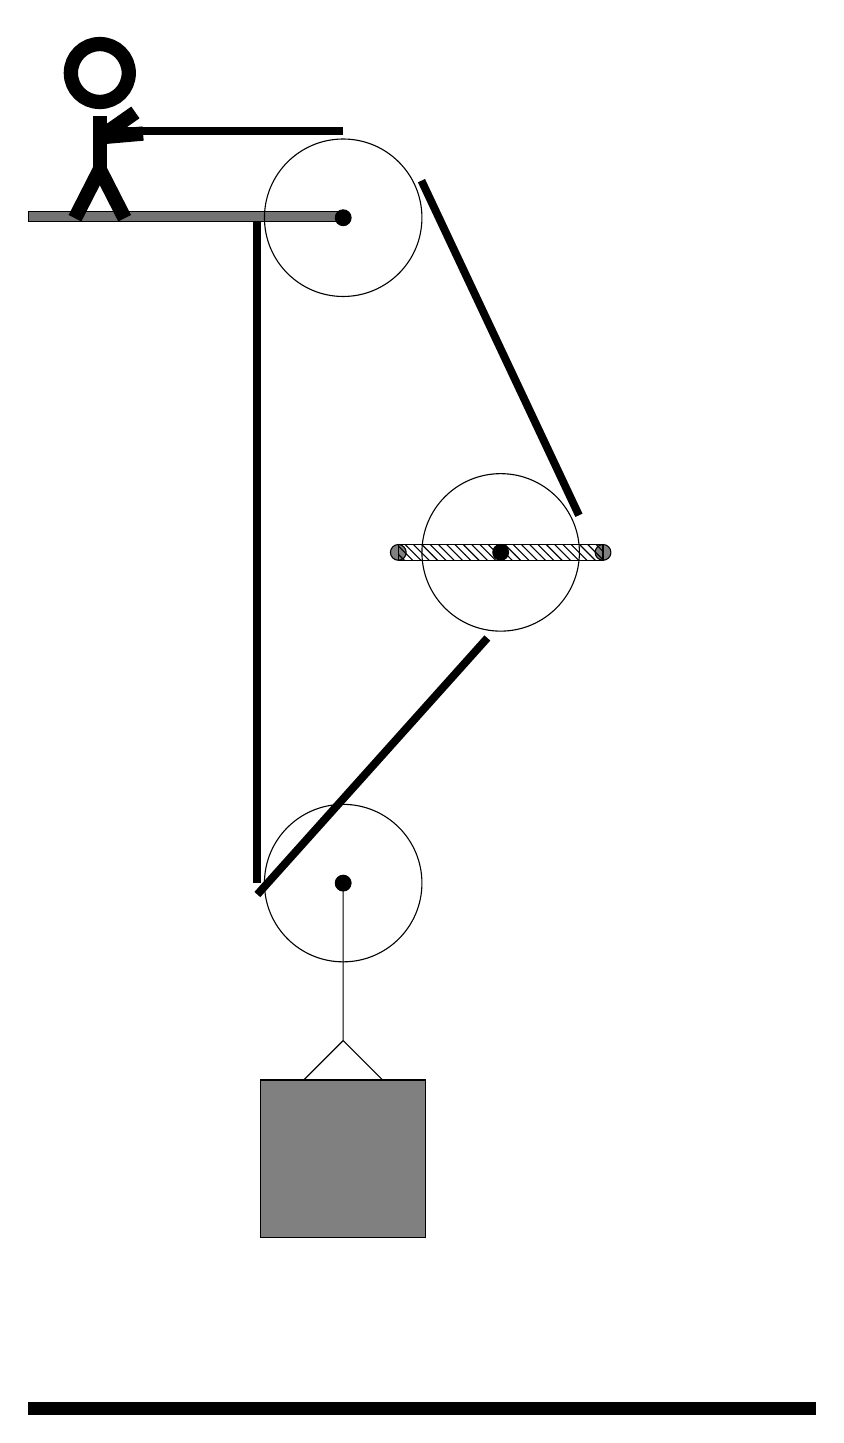
\begin{tikzpicture}
		%%%%% START %%%%%
		\draw[fill=black!55] (-2, 12) rectangle (2, 12.125);
		
		\draw (2, 3.6) circle (1);
		\draw[fill=black] (2, 3.6) circle (0.1);
		
		\draw (2, 12.05) circle (1);
		\draw[fill=black] (2, 12.05) circle (0.1);
		
		\draw[fill=white](4, 7.8) circle (1);
		\draw[fill=black] (4, 7.8) circle (0.1);
		\draw[fill=black!50] (2.7, 7.8) circle (0.1);
		\draw[fill=black!50] (5.3, 7.8) circle (0.1);
		\draw[pattern=north west lines, pattern color=black] (2.7, 7.9) rectangle (5.3, 7.7);
		
		\draw (2, 3.6) -- (2, 1.6) -- (1.5, 1.1) -- (2.5, 1.1) -- (2, 1.6);
		\draw[fill=black!50] (0.95, 1.1) rectangle (3.05, -0.9);
		
		\draw[line width=1mm] (0.9, 12) -- (0.9, 3.6);
		\centerarc[line width=1mm](2, 3.6)(180:330:1.1);
		\draw[line width=1mm](0.91, 3.455) -- (3.831, 6.713);
		\centerarc[line width=1mm](4, 7.8)(390:325:1.1);
		\draw[line width=1mm](4.994, 8.271) -- (2.994, 12.521);
		\centerarc[line width=1mm](2, 12.05)(30:90:1.1);
		\draw[line width=1mm](2, 13.15) -- (-1, 13.15);
		
		\node at (-1, 13.15) {\Strichmaxerl[10][-175][35]};
		
		\draw[fill=black] (-2, -3) rectangle (8, -3.15);
		%%%%% END %%%%%
	\end{tikzpicture}
\end{document}